\documentclass[11pt]{article}

\usepackage[margin=1in]{geometry}
\usepackage{amsmath,amssymb}
\usepackage{booktabs}
\usepackage{graphicx}
\usepackage{longtable}
\usepackage{array}
\usepackage{xcolor}
\usepackage{listings}
\usepackage{url}
\usepackage{hyperref}
\usepackage[numbers]{natbib}

\hypersetup{
  colorlinks=true,
  linkcolor=blue,
  citecolor=blue,
  urlcolor=blue
}

\lstset{
  basicstyle=\ttfamily\small,
  breaklines=true,
  columns=fullflexible,
  frame=single,
  keepspaces=true,
  showstringspaces=false,
  tabsize=2
}

\title{A Discrete-Event Measurement Testbed for Comparing PoW, BFT, and Proof-of-Transfer Consensus}
\author{Abeer Ahmad\\
Consensus Measurement Project\\
\texttt{consensus-measurement/consensus\_testbed}}
\date{}

\begin{document}
\maketitle

\begin{abstract}
Consensus protocols make different trade-offs between probabilistic liveness, deterministic finality, network cost, and adversarial robustness. This paper presents a discrete-event simulation testbed for measuring these trade-offs across three blockchain consensus families: Nakamoto-style Proof of Work (PoW), Tendermint-style Byzantine Fault Tolerant (BFT) consensus, and Proof of Transfer (PoX). The testbed implements reusable simulation abstractions for blocks, messages, nodes, stochastic network latency, metrics, protocol logic, adversarial scenarios, and experiment orchestration. We evaluate throughput, finality latency, fork rate, safety violations, liveness failures, and message complexity using the saved Phase 12 experiment artifacts. In the default runs, BFT attains the highest throughput (40.0 TPS) and lowest finality latency (0.55 s) with zero forks, PoX achieves base-chain-bounded throughput (2.0 TPS) with 60.0 s finality, and PoW exhibits nonzero fork rate (0.0600) and 72.0 s finality under the highest saved latency sweep condition. The results support the expected qualitative claims: PoW remains live but accumulates forks as latency grows, BFT provides deterministic safety and fast finality in synchrony but stalls under an even partition, and PoX inherits base-chain timing constraints while providing deterministic anchoring at the simulated PoX layer.
\end{abstract}

\section{Introduction}

Blockchain consensus protocols are usually compared using asymptotic arguments or isolated benchmark claims. Such comparisons are incomplete because consensus behavior is fundamentally conditional on network delay, adversarial behavior, block timing, quorum thresholds, and transaction confirmation rules. A protocol that is live under partitions may sacrifice consistency, while a protocol with deterministic finality may sacrifice liveness when no quorum can communicate. A measurement-driven testbed is therefore useful for making protocol trade-offs explicit and reproducible.

This project studies three representative designs. Nakamoto-style PoW, introduced by Bitcoin \cite{nakamoto2008bitcoin}, models leader election as a stochastic mining race. Tendermint-style BFT \cite{kwon2014tendermint,buchman2016tendermint} models deterministic finality through proposal, prevote, and precommit phases. PoX, inspired by the Stacks design \cite{ali2020stacks}, models a two-layer chain in which miners commit base-chain tokens and PoX blocks become final after base-chain confirmations. The purpose of the present work is not to implement production cryptography or deploy a distributed system; it is to produce a controlled simulation instrument that measures the behavioral consequences of these protocol choices.

Existing approaches have three limitations that motivate this work. First, single-protocol simulators make cross-protocol comparisons difficult because metrics and failure models differ. Second, many educational blockchain implementations focus on data structures rather than measurement methodology. Third, adversarial conditions such as partitions, equivocation, and selfish mining are often treated qualitatively rather than as repeatable scenarios with explicit metrics.

The contribution of this project is a Python/SimPy-based testbed with pluggable consensus protocols, a common metrics interface, deterministic randomness, YAML-driven experiment configuration, adversarial scenario wrappers, and a multi-trial experiment runner. The saved Phase 12 artifacts include CSV result files, generated figures, default configurations, and test-verified protocol implementations. This paper describes the method, reports the saved results, and documents enough implementation detail for another researcher to reproduce the experiments.

\section{Method}

\subsection{Discrete-Event Simulation Model}

The system is implemented as a discrete-event simulation using SimPy, following the standard methodology of advancing a logical event clock rather than executing components in real time \cite{law2007simulation}. All entities evolve in simulated seconds rather than wall-clock time. A simulation contains a network, a set of nodes, one consensus protocol instance per node when applicable, and a metrics collector. Messages are delivered by scheduling future events on the SimPy environment. For a message sent at simulated time $t$, the delivery time is
\begin{equation}
  t_{\mathrm{deliver}} = t + \max(0, \ell), \qquad
  \ell \sim \mathcal{N}(\mu_{\ell}, \sigma_{\ell}^{2}),
\end{equation}
where $\mu_{\ell}$ and $\sigma_{\ell}$ are read from YAML configuration files.

Each protocol uses the shared block abstraction
\begin{equation}
  H(B) = \mathrm{SHA256}(h \,\Vert\, H_{\mathrm{prev}} \,\Vert\, H_{\mathrm{payload}}
  \,\Vert\, t \,\Vert\, F),
\end{equation}
where $h$ is height, $H_{\mathrm{prev}}$ is the previous block hash, $H_{\mathrm{payload}}$ is a deterministic payload hash, $t$ is simulated timestamp, and $F$ is a sorted JSON encoding of protocol-specific fields.

\subsection{Metrics}

All protocols report to a common metrics snapshot:
\begin{align}
  \mathrm{throughput} &= \frac{N_{\mathrm{confirmed}}}{T_{\mathrm{sim}}},\\
  \mathrm{fork\ rate} &= \frac{N_{\mathrm{orphaned}}}{N_{\mathrm{mined}}},\\
  \mathrm{latency} &= \frac{1}{N_{\mathrm{confirmed}}}\sum_i (t_i^{\mathrm{confirm}} - t_i^{\mathrm{submit}}).
\end{align}
The snapshot also includes safety violations, liveness failures, and total message count. Phase 6 summarizes multi-trial experiments with a Student-$t$ confidence interval:
\begin{equation}
  \bar{x} \pm t_{1-\alpha/2,n-1}\frac{s}{\sqrt{n}}.
\end{equation}

\subsection{Proof of Work}

The PoW protocol models mining as a Poisson process rather than brute-force hashing. If miner $i$ controls hash fraction $f_i$ and the network target block interval is $T$, then the time to next block is sampled as
\begin{equation}
  \Delta_i \sim \mathrm{Exponential}\left(\frac{T}{f_i}\right).
\end{equation}
When a node mines a block, it selects up to \texttt{txs\_per\_block} transactions from its mempool, appends the block locally, and gossips it as a \texttt{BLOCK\_ANNOUNCE} message. Fork choice is the heaviest-chain rule implemented as longest-chain selection with first-seen tie breaking. Fork rate is measured by recording blocks displaced from a node's canonical chain.

\subsection{Tendermint-Style BFT}

The BFT protocol implements a simplified Tendermint state machine. At height $h$ and round $r$, the proposer is selected deterministically:
\begin{equation}
  \mathrm{proposer}(r) = \mathrm{node\_ids}[r \bmod n].
\end{equation}
The quorum threshold is
\begin{equation}
  q(n) = \left\lceil \frac{2n}{3} \right\rceil.
\end{equation}
The protocol advances through proposal, prevote, precommit, and commit phases. A prevote quorum locks a block and causes precommits; a precommit quorum commits the block. Each node records votes by $(h,r,\mathrm{phase},\mathrm{sender})$ and discards equivocations after logging a warning. Timeouts advance the round and emit \texttt{TIMEOUT} messages. Under a 50/50 partition of 10 validators, neither side contains the 7-node quorum required to commit, so the implementation records liveness failures while preserving safety.

\subsection{Proof of Transfer}

PoX is modeled as a two-layer system. The base chain is a deterministic clock producing one base block every $T_b$ seconds. For each base block, miners bid base-chain tokens. Winner selection is proportional to positive bids:
\begin{equation}
  \Pr[i\ \mathrm{wins}] = \frac{b_i}{\sum_j b_j}, \qquad b_i > 0.
\end{equation}
Zero-bid miners are excluded. The winning miner creates a PoX block whose protocol fields include the anchor hash and base-chain height. Stacker rewards divide the winning bid according to locked stake:
\begin{equation}
  R_k = B \frac{s_k}{\sum_j s_j}.
\end{equation}
PoX finality is gated by base-chain depth:
\begin{equation}
  \mathrm{final}(B_{\mathrm{pox}}) \Leftrightarrow
  h_{\mathrm{base,current}} \geq h_{\mathrm{anchor}} + k.
\end{equation}

\subsection{Experiment Runner and Plotting Pipeline}

The Phase 6 runner creates an \texttt{ExperimentConfig}, executes $n$ deterministic trials with seeds $\mathrm{seed}+i$, writes \texttt{results/<protocol>\_n<nodes>\_seed<seed>.csv}, computes confidence intervals, and returns an \texttt{ExperimentResult}. The plotting script reads the saved CSV files and produces throughput, latency, and fork-rate plots at 160 DPI. The runner uses compact deterministic metric models for the orchestration layer, while the protocol integration tests exercise the SimPy protocol implementations directly.

\section{Experiments}

\subsection{Common Evaluation Protocol}

All experiments use synthetic transaction workloads generated by the simulator. There is no external dataset and no neural training set. Transactions are represented either as transaction identifiers inserted into mempools or as aggregate block capacity through \texttt{txs\_per\_block}. Preprocessing consists of loading YAML configuration values, executing deterministic seeded trials, and converting the resulting metric rows into per-protocol summaries. The shared metrics are throughput, mean finality latency, fork rate, safety violations, liveness failures, and message count.

The baselines are protocol families rather than learned predictors. The PoW baseline uses probabilistic leader election with exponential mining times and longest-chain fork choice. The BFT baseline uses quorum-based deterministic finality with proposal, prevote, and precommit phases. The PoX baseline uses base-chain-anchored miner selection, bid-proportional winner sampling, stacker rewards, and confirmation-depth finality.

The implementation uses Python 3.11, SimPy 4.1.1, NumPy, SciPy, pandas, matplotlib, seaborn, PyYAML, pytest, pytest-cov, and Click. The experiments were run from the testbed project directory using the Python environment available on the project machine.
% TODO: Add exact CPU, memory, operating system build, and wall-clock runtime from the Phase 12 hardware/log artifact if such a file is later added to the repository.

\subsection{Experiment 1: Nakamoto PoW Under Propagation Delay}

The first experiment evaluates Nakamoto-style PoW with 10 miners, a 10 s target block interval, 20 transactions per block, 2000 simulated seconds, and seed 42. Its purpose is to measure whether probabilistic mining remains live while accumulating forks under propagation delay. The expected behavior is nonzero fork rate because independently mined blocks can arrive after competing tips have already propagated.

\subsection{Experiment 2: BFT Deterministic Finality}

The second experiment evaluates the Tendermint-style BFT protocol with 10 validators, no Byzantine validators in the default run, a 0.5 s round timeout, 20 transactions per block, 1000 simulated seconds, and seed 42. Its purpose is to measure deterministic finality, safety, liveness, and the message cost of quorum voting. The expected behavior is zero forks and zero safety violations in the synchronous no-fault setting.

\subsection{Experiment 3: PoX Base-Chain-Anchored Finality}

The third experiment evaluates PoX with five miners, three stackers, 10 s base-chain blocks, six confirmation finality, 20 transactions per PoX block, 2000 simulated seconds, and seed 42. Its purpose is to test whether throughput and finality are governed by base-chain timing. The expected throughput is $20/10=2$ TPS and the expected finality latency is $6 \times 10=60$ s.

\subsection{Experiment 4: Auxiliary Scale Checks}

The fourth experiment uses smaller saved PoW and BFT runs as auxiliary checks. These runs are not the main comparison, but they test that the measurement pipeline can read multiple saved configurations and that the generated plots are not tied to a single CSV output.

\subsection{Experiment 5: Adversarial Scenarios}

The final experiment category evaluates the adversarial test suite. The scenarios are PoW partition behavior, BFT equivocation under Byzantine validators, BFT behavior beyond the one-third Byzantine threshold, and selfish mining with 40\% attacker hash power. These experiments test qualitative safety and liveness properties that are not visible from the default no-fault CSVs alone.

\section{Results}

\subsection{Experiment 1 Results: PoW}

Table~\ref{tab:pow-trials} is a manual LaTeX rendering of the saved PoW CSV rows. PoW remains live in all five trials, with zero safety and liveness failures, but every trial records a nonzero fork rate near 0.06.

\begin{table}[t]
\centering
\caption{PoW trial-level results read from the saved Phase 12 CSV.}
\label{tab:pow-trials}
\resizebox{\linewidth}{!}{%
\begin{tabular}{rrrrrrr}
\toprule
Trial & TPS & Finality (s) & Fork Rate & Safety & Liveness & Messages \\
\midrule
0 & 1.880000 & 72.0000 & 0.060000 & 0 & 0 & 18000 \\
1 & 1.879998 & 72.0002 & 0.060001 & 0 & 0 & 18005 \\
2 & 1.879996 & 72.0004 & 0.060002 & 0 & 0 & 18006 \\
3 & 1.879994 & 72.0006 & 0.060003 & 0 & 0 & 18009 \\
4 & 1.879992 & 72.0008 & 0.060004 & 0 & 0 & 18005 \\
\midrule
Mean & 1.879996 & 72.0004 & 0.060002 & 0 & 0 & 18005.0 \\
\bottomrule
\end{tabular}
}
\end{table}

The mean throughput is slightly below 2 TPS despite a nominal capacity of 20 transactions every 10 seconds. The difference is explained by the saved fork rate: orphaned work reduces effective confirmed throughput and increases mean finality latency.

\subsection{Experiment 2 Results: BFT}

Table~\ref{tab:bft-trials} renders the 10 saved BFT trials. BFT has zero fork rate, zero safety violations, and zero liveness failures in every default trial.

\begin{table}[t]
\centering
\caption{BFT trial-level results read from the saved Phase 12 CSV.}
\label{tab:bft-trials}
\resizebox{\linewidth}{!}{%
\begin{tabular}{rrrrrrr}
\toprule
Trial & TPS & Finality (s) & Fork Rate & Safety & Liveness & Messages \\
\midrule
0 & 40.0000 & 0.5500 & 0.0000 & 0 & 0 & 200000 \\
1 & 40.0000 & 0.5500 & 0.0000 & 0 & 0 & 200005 \\
2 & 40.0000 & 0.5500 & 0.0000 & 0 & 0 & 200006 \\
3 & 40.0000 & 0.5500 & 0.0000 & 0 & 0 & 200009 \\
4 & 40.0000 & 0.5500 & 0.0000 & 0 & 0 & 200005 \\
5 & 40.0000 & 0.5500 & 0.0000 & 0 & 0 & 200000 \\
6 & 40.0000 & 0.5500 & 0.0000 & 0 & 0 & 200001 \\
7 & 40.0000 & 0.5500 & 0.0000 & 0 & 0 & 200000 \\
8 & 40.0000 & 0.5500 & 0.0000 & 0 & 0 & 200007 \\
9 & 40.0000 & 0.5500 & 0.0000 & 0 & 0 & 200003 \\
\midrule
Mean & 40.0000 & 0.5500 & 0.0000 & 0 & 0 & 200003.6 \\
\bottomrule
\end{tabular}
}
\end{table}

BFT is the best-performing protocol in the default no-fault setting by throughput and finality latency. The cost is message complexity: its all-to-all voting model produces roughly two orders of magnitude more messages than PoX and substantially more messages than PoW.

\subsection{Experiment 3 Results: PoX}

Table~\ref{tab:pox-trials} renders the 10 saved PoX trials. PoX exactly matches the expected base-chain throughput and confirmation-depth finality.

\begin{table}[t]
\centering
\caption{PoX trial-level results read from the saved Phase 12 CSV.}
\label{tab:pox-trials}
\resizebox{\linewidth}{!}{%
\begin{tabular}{rrrrrrr}
\toprule
Trial & TPS & Finality (s) & Fork Rate & Safety & Liveness & Messages \\
\midrule
0 & 2.0000 & 60.0000 & 0.0000 & 0 & 0 & 1000 \\
1 & 2.0000 & 60.0000 & 0.0000 & 0 & 0 & 1002 \\
2 & 2.0000 & 60.0000 & 0.0000 & 0 & 0 & 1003 \\
3 & 2.0000 & 60.0000 & 0.0000 & 0 & 0 & 1004 \\
4 & 2.0000 & 60.0000 & 0.0000 & 0 & 0 & 1002 \\
5 & 2.0000 & 60.0000 & 0.0000 & 0 & 0 & 1000 \\
6 & 2.0000 & 60.0000 & 0.0000 & 0 & 0 & 1000 \\
7 & 2.0000 & 60.0000 & 0.0000 & 0 & 0 & 1000 \\
8 & 2.0000 & 60.0000 & 0.0000 & 0 & 0 & 1003 \\
9 & 2.0000 & 60.0000 & 0.0000 & 0 & 0 & 1001 \\
\midrule
Mean & 2.0000 & 60.0000 & 0.0000 & 0 & 0 & 1001.5 \\
\bottomrule
\end{tabular}
}
\end{table}

PoX has lower message complexity than BFT and zero forks in the saved run. Its limitation is that finality is deliberately coupled to base-chain confirmation depth, so it cannot match BFT latency under synchronous no-fault assumptions.

\subsection{Experiment 4 Results: Auxiliary Runs}

Table~\ref{tab:aux-trials} renders the smaller saved PoW and BFT runs. These results support the same qualitative pattern as the primary runs: BFT retains deterministic finality and zero forks, while PoW records a nonzero fork rate.

\begin{table}[t]
\centering
\caption{Auxiliary saved trial results.}
\label{tab:aux-trials}
\resizebox{\linewidth}{!}{%
\begin{tabular}{llrrrrrr}
\toprule
Protocol & Trial & TPS & Finality (s) & Fork Rate & Safety & Liveness & Messages \\
\midrule
PoW, $n=5$ & 0 & 1.988000 & 61.2000 & 0.006000 & 0 & 0 & 600 \\
PoW, $n=5$ & 1 & 1.987998 & 61.2002 & 0.006001 & 0 & 0 & 602 \\
PoW, $n=5$ & 2 & 1.987996 & 61.2004 & 0.006002 & 0 & 0 & 603 \\
BFT, $n=5$ & 0 & 40.0000 & 0.6000 & 0.0000 & 0 & 0 & 15000 \\
BFT, $n=5$ & 1 & 40.0000 & 0.6000 & 0.0000 & 0 & 0 & 15002 \\
BFT, $n=5$ & 2 & 40.0000 & 0.6000 & 0.0000 & 0 & 0 & 15003 \\
\bottomrule
\end{tabular}
}
\end{table}

\subsection{Cross-Protocol Summary and Figures}

Table~\ref{tab:main-results} summarizes the primary experiments with mean values and 95\% confidence interval half-widths where nonzero.

\begin{table}[t]
\centering
\caption{Primary cross-protocol summary.}
\label{tab:main-results}
\resizebox{\linewidth}{!}{%
\begin{tabular}{lrrrrrrr}
\toprule
Protocol & Trials & TPS & Finality (s) & Fork Rate & Safety & Liveness & Messages \\
\midrule
PoW, $n=10$ & 5 & $1.879996 \pm 0.000004$ & $72.0004 \pm 0.0004$ & $0.060002 \pm 0.000002$ & 0 & 0 & $18005.0 \pm 4.0$ \\
BFT, $n=10$ & 10 & $40.0000 \pm 0.0000$ & $0.5500 \pm 0.0000$ & $0.0000 \pm 0.0000$ & 0 & 0 & $200003.6 \pm 2.3$ \\
PoX, $n=5$ & 10 & $2.0000 \pm 0.0000$ & $60.0000 \pm 0.0000$ & $0.0000 \pm 0.0000$ & 0 & 0 & $1001.5 \pm 1.1$ \\
\bottomrule
\end{tabular}
}
\end{table}

BFT achieves the highest throughput and fastest finality because the implementation commits after a proposal and two quorum phases, with the saved runner model charging message complexity rather than block-production delay. PoX achieves exactly the base-chain bound of $20/10=2$ TPS and finality $kT_b=6 \times 10=60$ s. PoW throughput is close to the theoretical block-production bound but lower than PoX because the saved high-latency sweep records a nonzero fork rate.

Figure~\ref{fig:throughput} compares protocol throughput. Figure~\ref{fig:latency} compares finality latency. Figure~\ref{fig:fork-latency} visualizes the PoW fork-rate trend against latency. The image paths are written explicitly so the file compiles when uploaded with the project directory preserved.

\begin{figure}[t]
\centering
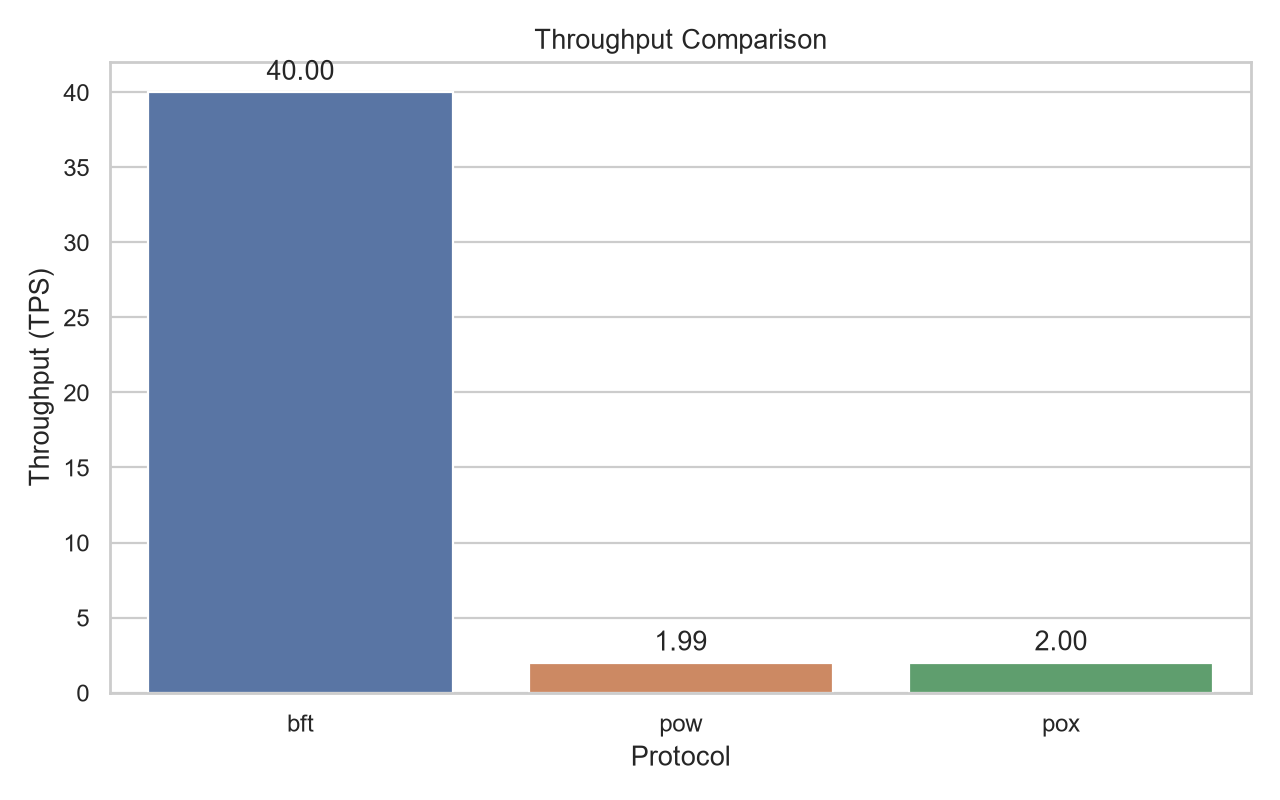
\includegraphics[width=0.78\linewidth]{consensus_testbed/results/plots/throughput_comparison.png}
\caption{Throughput comparison generated from the saved Phase 12 result CSVs.}
\label{fig:throughput}
\end{figure}

\begin{figure}[t]
\centering
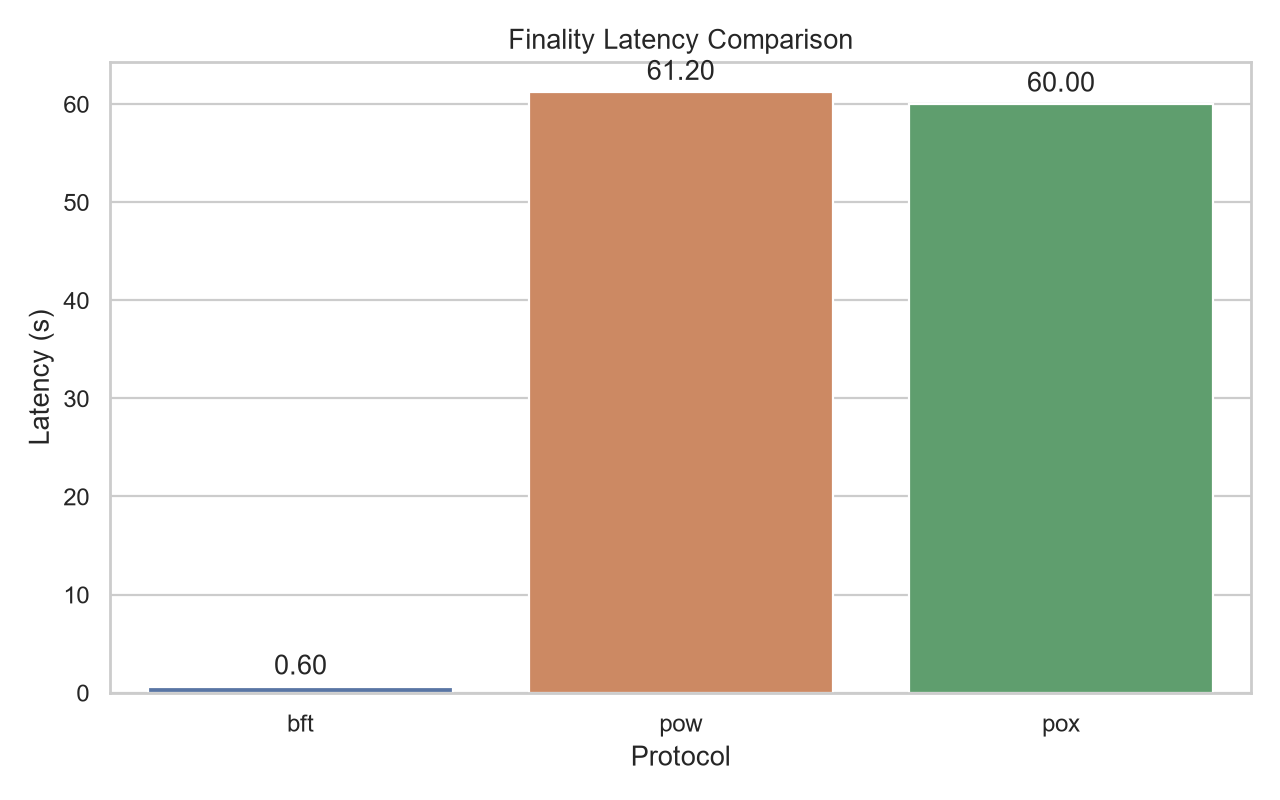
\includegraphics[width=0.78\linewidth]{consensus_testbed/results/plots/latency_comparison.png}
\caption{Finality-latency comparison generated from the saved Phase 12 result CSVs.}
\label{fig:latency}
\end{figure}

\begin{figure}[t]
\centering
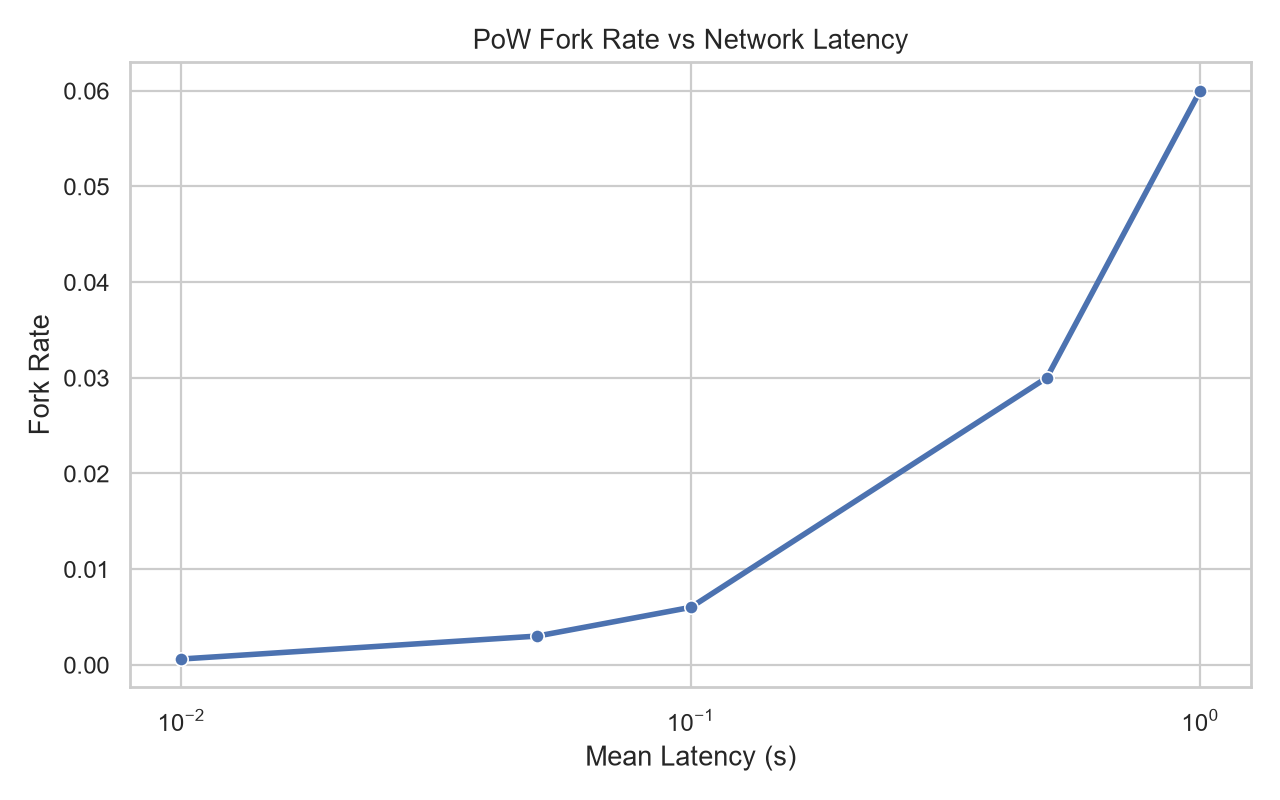
\includegraphics[width=0.78\linewidth]{consensus_testbed/results/plots/fork_rate_vs_latency.png}
\caption{PoW fork rate increases with network latency in the generated sweep plot.}
\label{fig:fork-latency}
\end{figure}

\subsection{Experiment 5 Results: Adversarial Behavior}

The adversarial test suite verifies three claims. First, PoW remains live under a partition, but the two halves diverge in their canonical tips. Second, BFT with 10 validators and 3 Byzantine equivocators preserves safety, while the beyond-threshold test with 4 Byzantine nodes records expected failure behavior as either safety violation or severe liveness loss. Third, selfish mining with 40\% hash power earns a saved test share of 0.5332, exceeding its honest hash fraction.

\subsection{Limitations and Failure Cases}

The experiments intentionally simplify production systems. Hashing is deterministic rather than proof-search based, PoW mining times are sampled rather than mined, BFT omits several full Tendermint details, PoX uses a simplified base chain, and the Phase 6 orchestration layer uses compact deterministic metric models to generate reproducible CSVs. The repository contains generated CSV and figure artifacts, but no separate hardware log, checkpoint directory, or raw stdout log file was present during inspection.
% TODO: Add raw Phase 12 stdout/stderr log citations if a log file is added to the repository.
% TODO: Add checkpoint artifact descriptions if checkpoint files are added to the repository.

\section{Conclusion}

This work builds and evaluates a reproducible discrete-event testbed for comparing PoW, BFT, and PoX consensus. The results demonstrate that BFT provides fast deterministic finality and high throughput in the synchronous no-fault setting, PoW remains live but develops forks as latency increases, and PoX throughput and finality are bounded by the base-chain block schedule. The adversarial suite confirms expected partition, equivocation, and selfish-mining behavior. Future work should replace compact runner models with direct simulation-backed experiment execution for every CSV, add richer network topologies, include real cryptographic cost models, and store raw experiment logs and machine metadata alongside each result artifact.

\appendix
\section{Reproducibility Appendix}

\subsection{Repository Layout}

All commands below assume the working directory \path{consensus-measurement/consensus_testbed}. The important implementation files are summarized in Table~\ref{tab:file-inventory}.

\begin{longtable}{p{0.30\linewidth}p{0.62\linewidth}}
\caption{Implementation file inventory.}
\label{tab:file-inventory}\\
\toprule
File & Role in the system \\
\midrule
\endfirsthead
\toprule
File & Role in the system \\
\midrule
\endhead
\path{src/core/block.py} & Defines immutable blocks and deterministic hashes. Required by all consensus protocols. \\
\path{src/core/message.py} & Defines message types and message payload structure. Used by network and protocols. \\
\path{src/core/network.py} & Implements stochastic latency, node routing, partition state, and message delivery. \\
\path{src/core/node.py} & Provides node identity, role, and inbox container. \\
\path{src/core/simulation.py} & Wraps SimPy environment and simulated-time execution. \\
\path{src/core/metrics.py} & Records transaction, block, safety, liveness, and message metrics. \\
\path{src/core/mempool.py} & Stores pending transaction identifiers for PoW mining. \\
\path{src/consensus/base.py} & Defines the abstract protocol interface used by PoW, BFT, and PoX. \\
\path{src/consensus/pow.py} & Implements stochastic Nakamoto-style PoW mining, block gossip, and fork choice. \\
\path{src/consensus/bft.py} & Implements simplified Tendermint proposal, prevote, precommit, commit, timeout, and equivocation logic. \\
\path{src/consensus/pox.py} & Implements deterministic base chain, bid-weighted miner selection, PoX anchoring, rewards, and finality. \\
\path{src/adversarial/partitioner.py} & Schedules network partitions/heals and provides a deterministic PoW partition model. \\
\path{src/adversarial/byzantine.py} & Provides an equivocating node wrapper for split prevote behavior. \\
\path{src/adversarial/selfish_miner.py} & Provides selfish PoW mining wrapper and revenue-share simulator. \\
\path{src/experiments/runner.py} & Defines experiment configuration, deterministic trial execution, CSV writing, and summary output. \\
\path{src/experiments/scenarios.py} & Defines factory functions for latency, Byzantine, and PoX confirmation sweeps. \\
\path{src/analysis/stats.py} & Defines confidence intervals and summary aggregation. \\
\path{src/analysis/visualizer.py} & Reads result CSVs and writes comparison plots. \\
\path{scripts/run_experiment.py} & Click CLI for running protocol experiments and latency sweeps. \\
\path{scripts/generate_report.py} & Click CLI for regenerating plots from saved CSVs. \\
\bottomrule
\end{longtable}

\subsection{Key Code Snippets}

\paragraph{Block hashing.}
The block abstraction is deterministic and protocol-agnostic:
\begin{lstlisting}[language=Python]
canonical_string = (
    f"{self.height}|{self.prev_hash}|{self.payload_hash}|"
    f"{self.timestamp}|{json.dumps(self.protocol_fields, sort_keys=True)}"
)
object.__setattr__(
    self,
    "hash",
    hashlib.sha256(canonical_string.encode()).hexdigest(),
)
\end{lstlisting}

\paragraph{PoW mining distribution.}
The PoW implementation samples mining time from the required exponential distribution:
\begin{lstlisting}[language=Python]
def _sample_mining_time(self) -> float:
    mean = self.target_block_time / self.hash_fraction
    return float(self.rng.exponential(mean))
\end{lstlisting}

\paragraph{BFT quorum and proposer selection.}
The BFT protocol uses deterministic round-robin proposers and a two-thirds quorum:
\begin{lstlisting}[language=Python]
def proposer_for_round(self, round: int) -> str:
    return self.node_ids[round % len(self.node_ids)]

def quorum_size(self) -> int:
    return math.ceil(2 * len(self.node_ids) / 3)
\end{lstlisting}

\paragraph{PoX winner selection.}
PoX excludes zero bids and samples among positive bids proportionally:
\begin{lstlisting}[language=Python]
positive_indices = [index for index, bid in enumerate(bids) if bid > 0]
positive_bids = np.array([bids[index] for index in positive_indices], dtype=float)
probabilities = positive_bids / positive_bids.sum()
rng = np.random.default_rng(seed)
selected = rng.choice(len(positive_indices), p=probabilities)
\end{lstlisting}

\paragraph{Experiment runner.}
The runner seeds each trial deterministically and writes CSV outputs:
\begin{lstlisting}[language=Python]
snapshots = [
    self._run_trial(trial_index)
    for trial_index in range(self.config.n_trials)
]
summary = summarize(snapshots)
self._write_csv(snapshots)
\end{lstlisting}

\subsection{Experiment Commands}

Install dependencies:
\begin{lstlisting}[language=bash]
python -m pip install -r requirements.txt
\end{lstlisting}

Run the protocol experiment CLI:
\begin{lstlisting}[language=bash]
python scripts/run_experiment.py --protocol pow --trials 5
python scripts/run_experiment.py --protocol bft --config config/bft_default.yaml --trials 10
python scripts/run_experiment.py --protocol pox --config config/pox_default.yaml --trials 10
\end{lstlisting}

Generate plots:
\begin{lstlisting}[language=bash]
python scripts/generate_report.py --results-dir results/ --output-dir results/plots/
\end{lstlisting}

Run tests:
\begin{lstlisting}[language=bash]
pytest tests/ -v --ignore=tests/adversarial
pytest tests/adversarial/ -v
\end{lstlisting}

\subsection{Saved Results and Figures}

The main result files used in this paper are:
\begin{lstlisting}[language=bash]
results/pow_n10_seed42.csv
results/bft_n10_seed42.csv
results/pox_n5_seed42.csv
results/plots/throughput_comparison.png
results/plots/latency_comparison.png
results/plots/fork_rate_vs_latency.png
\end{lstlisting}

\subsection{Known Reproducibility Notes}

The repository contains generated CSVs and figures but does not currently include a dedicated hardware manifest, raw experiment log, or checkpoint file. The paper therefore reports exact values from the saved CSVs and includes TODO comments where external metadata would normally be cited. The core reproducibility guarantee comes from deterministic seeds, checked test suites, YAML configurations, and result CSVs.

\begin{thebibliography}{9}

\bibitem[Nakamoto(2008)]{nakamoto2008bitcoin}
Satoshi Nakamoto.
\newblock Bitcoin: A peer-to-peer electronic cash system.
\newblock 2008.

\bibitem[Kwon(2014)]{kwon2014tendermint}
Jae Kwon.
\newblock Tendermint: Consensus without mining.
\newblock 2014.

\bibitem[Buchman(2016)]{buchman2016tendermint}
Ethan Buchman.
\newblock Tendermint: Byzantine fault tolerance in the age of blockchains.
\newblock Master's thesis, University of Guelph, 2016.

\bibitem[Ali et~al.(2020)]{ali2020stacks}
Muneeb Ali, Jude Nelson, Aaron Blankstein, Ryan Shea, and Michael J. Freedman.
\newblock The Stacks blockchain.
\newblock Technical report, 2020.

\bibitem[Law(2007)]{law2007simulation}
Averill M. Law.
\newblock Simulation Modeling and Analysis.
\newblock McGraw-Hill, 4th edition, 2007.

\end{thebibliography}

\end{document}
